\documentclass[b5paper, 11pt, norsk]{MScthesisITEM}

% this package is just to generate text for demo-purposes
\usepackage[norsk]{babel}
%\usepackage{blindtext}
\usepackage{parskip}


\title{Awareness Communication and \newlinetitle Distribution Service for
Hospitals} % The title of your assignement; NB use \newlinetitle to start a newline
\author{Veronica Sund \\ \newlinetitle Monika Hafredal} % Your firstname and lastname
\professor{Lill Kristiansen, ITEM} % Affiliation = ITEM for instance
\supervisor{Joakim Klemets, ITEM}
\date{Desember 2013}

%% Uncomment the following in case you want subfigures; note that there will be a warning for the caption package
% \let\subcaption\undefined
% \let\subfloat\undefined
% \usepackage[bf]{caption}
% \usepackage{subcaption}

\DeclareGraphicsExtensions{.pdf,.jpg}
\graphicspath{{./figs/}}



\loadglsentries{glossary}
\makeglossaries

\begin{document}
\selectlanguage{norsk}
\pagenumbering{roman}
\pagestyle{plain}

%% Only for the project
\titleITEM

%% Only for the master's thesis; for the project report the description is taken from It's Learning and added by the department
% \selectlanguage{english} % Change to 'norsk' if you are writing in Norwegian
% \input{problem_description}
% \cleardoublepage

%% There must be an abstract in English, even though the main text is in Norwegian
\selectlanguage{norsk}
%\pagestyle{empty}
\begin{abstract}

\noindent
To maintain awareness of colleagues' work is essential for good coordination. Nurses receive information necessary to maintain such awareness through external interrupts. These disruptions, in addition to the already interrupted-driven environment they work in.
This research paper looks at the nurse call system at St. Olav's Hospital in Trondheim. We have seen how this works today, how nurses maintain awareness at work item and how it interrupted-driven environment affects their work.


%\Blindtext[5][1]
\end{abstract}
\cleardoublepage

%% Only for the master's thesis; if the main text is in English and you can write Norwegian, there must be an abstract in Norwegian as well.A
% \selectlanguage{norsk}
% \pagestyle{empty}
\renewcommand{\abstractname}{Sammendrag}
\begin{abstract}
\noindent Sikkerheten til nesten all offentlig nøkkel-kryptografi er basert på et vanskelig beregnbarhetsproblem. Mest velkjent er problemene med å faktorisere heltall i sine primtallsfaktorer, og å beregne diskrete logaritmer i endelige sykliske grupper. I de to siste tiårene, har det imidlertid dukket opp en rekke andre offentlig nøkkel-systemer, som baserer sin sikkerhet på helt andre type problemer. Et lovende forslag, er å basere sikkerheten på vanskeligheten av å løse store likningsett av flervariable polynomlikninger. En stor utfordring ved å designe slike offentlig nøkkel-systemer, er å integrere en effektiv ``falluke'' (trapdoor) inn i likningssettet. En ny tilnærming til dette problemet ble nylig foreslått av Gligoroski m.f., hvor de benytter konseptet om kvasigruppe-strengtransformasjoner (quasigroup string transformations). I denne masteroppgaven beskriver vi en metodikk for å identifisere sterke og svake nøkler i det nylig foreslåtte multivariable offentlig nøkkel-signatursystemet MQQ-SIG, som er basert på denne idéen.

Vi har gjennomført et stort antall eksperimenter, basert på Gröbner basis angrep, for å klassifisere de ulike parametrene som bestemmer nøklene i MQQ-SIG. Våre funn viser at det er store forskjeller i viktigheten av disse parametrene. Metodikken består i en klassifisering av de forskjellige parametrene i systemet, i tillegg til en innføring av konkrete kriterier for hvilke nøkler som bør velges. Videre, har vi identifisert et unødvendig krav i den originale spesifikasjonen, som krevde at kvasigruppene måtte oppfylle et bestemt kriterie. Ved å fjerne denne betingelsen, kan nøkkel-genererings-algoritmen potensielt øke ytelsen med en stor faktor. Basert på alt dette, foreslår vi en ny og forbedret nøkkel-genereringsalgoritme for MQQ-SIG, som vil generere sterkere nøkler og være mer effektiv enn den originale nøkkel-genereringsalgoritmen.  
\end{abstract}
% \cleardoublepage

%\selectlanguage{norsk}% Change to 'norsk' if you are writing in Norwegian
%\pagestyle{empty}
\begin{abstract}

\noindent
To maintain awareness of colleagues' work is essential for good coordination. Nurses receive information necessary to maintain such awareness through external interrupts. These disruptions, in addition to the already interrupted-driven environment they work in.
This research paper looks at the nurse call system at St. Olav's Hospital in Trondheim. We have seen how this works today, how nurses maintain awareness at work item and how it interrupted-driven environment affects their work.


%\Blindtext[5][1]
\end{abstract}

%\renewcommand{\abstractname}{Preface}
\begin{abstract}

\noindent
Denne prosjektoppgaven er skrevet ved Institutt for Telematikk (ITEM) ved Norges Teknisk-Naturvitenskapelige Universitet (NTNU), høsten 2013. Forfatterene har fulgt studieprogrammet Kommunikasjonteknologi innen retingen Nett og Tjenester, med fordypning innen Telematikk og Samfunn. 

\noindent
Bakgrunnsinformasjon og -data er skaffet gjennom studier av tidligere arbeid, samt workshops med test og evaluering av prototype. 

\noindent
Vi vil først takke professor Lill Kristiansen (ITEM), ansvarlig professor for oppgaven, for gode innspill underveis. Vi ønsker også å rette en stor takk til vår veileder Ph.D. kandidat Joakim Klemets, ved ITEM, for gode tilbakemeldinger, konstruktiv kritikk og støtte underveis i arbeidet. Joakim la også stor innsats i å skaffe deltagere til workshopene.

\noindent
Vi vil også takke Terje Røsand ved Norsk Senter for Elektronisk Pasientjournal (NSEP) for gode videoopptak av workshopene, og god veiledning i forkant av disse. Til sist vil vi takke alle som har brukt tid på å hjelpe oss å lese korrektur på oppgaven.

\centering

Trondheim, 11. desember 2013\\
Veronica Sund\\
Monika Hafredal

%\blindtext 
\end{abstract}
\cleardoublepage

% similarly you may add a separate acknowledgments page

\tableofcontents*
\cleardoublepage

%% include if relevant
%\listoffigures
\cleardoublepage

%% include if relevant
%\listoftables
\cleardoublepage

%% include if relevant
%\listofalgorithms
%\addcontentsline{toc}{chapter}{List of Algorithms}
\cleardoublepage

%% include if relevant
%\printglossary[title=List of Symbols, style=long]
\cleardoublepage
%\glsaddall[]

%% include if relevant
%\printglossary[title=List of Acronyms,type=\acronymtype] % prints just the list of acronyms
\cleardoublepage

\pagenumbering{arabic}
\pagestyle{ruled}
%\include{example_chapter}
\chapter{Bakgrunn}
\label{chp:bakgrunn}

Oppsummering av tidligere arbeid


\chapter{Teori}
\label{chp:teori}


Vi vil i dette kapittelet presentere teori relevant for vår forskning. Denne teorien er et resultat av kvalitative literaturstudier, en metode nærmere beskrevet i kapittel \ref{chp:forskningsmetode}. Vi har valgt å fokusere på temaer vi mener er sentrale for spørsmålene vi søker svar på. Da vår oppgave omhandler et system som skal støtte samarbeid i et høyst dynamisk miljø, inneholder denne delen  både menneskelige og organisatoriske aspekter, samt teori knyttet til design og utvikling av slike systemer.

\section{Kognitiv distribusjon og kapasitet}
\label{chp: kognisjon}

Ofte vil arbeidsaktiviteter bestå av flere sammenflettede oppgaver i en gitt tidsramme. Jo lenger tid det tar å utføre en oppgave, jo større sjanse er det for at andre oppgaver eller handlinger må utføres i løpet av denne perioden. Disse oppgavene kan ha ulik avbruddsverdi - prioritet, personlig- eller sosial viktighet, hastegrad ol. \cite{Rogers94}. 
Da CSCW kom mot slutten av 80-tallet, oppsto utfordringene om hvordan datasystemer bør designes for å støtte grupper av individer som kommuniserer og arbeider sammen \cite{Rogers94}. 

\tikzstyle{mybox} = [draw=black, fill=white, very thick,
    rectangle, inner sep=10pt, inner ysep=20pt, rounded corners]
\tikzstyle{fancytitle} =[fill=black, text=white]
\begin{tikzpicture}
\node [mybox] (box){%
    \begin{minipage}{0.9\textwidth}
     Computer-Supported Cooperative Work er et tverrfaglig område hvor forskere studerer hvordan grupper av samarbeidende mennesker jobber, og hvordan teknologi kan være til støtte for arbeidet. CSCW-teknologi defineres som PC-baserte systemer som støtter grupper av mennesker engasjert i en felles oppgave, eller med et felles mål, og som gir et grensesnitt til det delte miljøet (Ellis (1991)) \nocite{Ellis91}.
    \end{minipage}
};
\node[fancytitle, rounded corners, right=10pt] at (box.north west) {CSCW};
\end{tikzpicture}%


\noindent
Gitt at mange arbeidsaktiviteter er kognitive, de krever tenkning, problemløsing og evne til å forutse og ta beslutninger, argumenterer Rogers og Ellis (1994) for at det kreves en forståelse for hvordan disse aktivitetene utføres for å kunne designe datasystemer som kan støtte både kognitive aktiviteter og sosial interaksjon.

\tikzstyle{mybox} = [draw=black, fill=white, very thick,
    rectangle, inner sep=10pt, inner ysep=20pt, rounded corners]
\tikzstyle{fancytitle} =[fill=black, text=white]
\begin{tikzpicture}
\node [mybox] (box){%
    \begin{minipage}{0.9\textwidth}
     Det som har med erkjennelse, oppfatning og tenkning å gjøre. I filosofi og psykologi opptrer ofte uttrykket 'kognitiv' som motsetning til det følelsesmessige eller intuitive. Et kognitivt system er et som kan behandle en viss type informasjon, for eksempel sanseinntrykk, minner, tanker eller språk. Menneskehjernen regnes som et eksempel på et kognitivt system (Malt et al. (2013), Store medisinske leksikon).
    \end{minipage}
};
\node[fancytitle, rounded corners, right=10pt] at (box.north west) {Kognitiv};
\end{tikzpicture}%

\subsection{Kognitiv kapasitet}
“Stacking” defineres av Ebright (2010) som den usynlige beslutningsprosessen sykepleiere utfører om hva, hvordan og når de skal gi pleie til en tildelt gruppe pasienter. Stadige endringer i omgivelser og informasjonsflyt resulterer i en kontinuerlig re-prioritering av hvilke oppgaver man skal gjøre når. Dette kombinert med avbrytelser fra omgivelsene, kan resultere i en kognitiv belastning som kan hemme oppmerksomheten. Parker og Coiera (2000) hevder at en begrensende faktor i enhver kommunikasjonsanalyse er den kognitive kapasiteten individer har til å gjennomføre sitt arbeid, da studier har vist at feil og ineffektivitet er et resultat av at denne kapasiteten overskrides. Kunnskap om menneskets hukommelse hevdes å være nøkkelen til å forstå hvilke krav som bør settes til teknologi brukt i slike omgivelser. Det skilles normalt mellom langtids- og korttidsminne. Den passive kunnskapen man besitter ligger i langtidsminnet, for eksempel medisinske fakta eller viktige datoer, mens kortidsminnet, eller arbeidsminnet, er den bevisste delen av minnet som aktivt behandler informasjon. Arbeidsminnet har begrenset kapasitet og varighet, og lar seg raskt forstyrre av distraksjoner og avbrytelser. Coiera og Tombs (1998) \nocite{Coiera98} antyder at synkron kommunikasjon, ansikt-til-ansikt eller per telefon, foretrekkes fordi det gir en umiddelbar bekreftelse på at en beskjed er mottatt. Dersom man ønsker å gi en beskjed eller et ansvar videre, vil usikkerheten om beskjeden er mottatt bli liggende i arbeidsminnet frem til man får en bekreftelse fra mottaker. 




\section{Awareness}
\label{chp: awareness}

Et sykehus er en organisasjon hvor vi finner mange informasjonskilder, plutselig stress, rutinearbeid og ansatte som stadig er på forskjellige steder. Dette gjør at kommunikasjon er svært viktig for å sikre god pasientomsorg og -sikkerhet\cite{Klemets12}. Uttrykket funksjonsredundans (av det engelske 'redundancy of function') betyr at kunnskap om situasjonen til en hver tid er delt, og overlappende mellom medlemmene i gruppen.\cite{KlemetsRedundancy} Denne typen kunnskap kalles gjerne for bevissthet, og er et konsept med stadig større betydning, spesielt med tanke på CSCW \cite{Dourish92}. En slik bevissthet om andres aktiviteter er avgjørene for å sikre et vellykket samarbeid og god koordinasjon\cite{KlemetsRedundancy}. 

\subsubsection{Definisjoner og konseptualiseringer}
Bevissthet er et svært uklart og komplekst konsept med mange definisjoner og konseptualiseringer \cite{KlemetsRedundancy}\cite{Gutwin04}\cite{Schmidt02}. Begrepet bevissthet brukes i stadig flere sammenhenger, og mange forskere blir stedig mindre komfortable med å bruke begrepet i seg selv. For å komme til en slags konseptuell klarhet i hva bevissthet skal bety må vi innse at det ikke gir mening å se på bevissthet noe i seg selv, men må referere til en persons bevissthet \emph{om} noe \cite{Schmidt02}. Dermed har vi fått konsepter som blant annet sosial, eller kontekstformidlet sosial bevissthet \cite{Bardram04}, generell bevissthet\cite{Gross13}, romlig og tidsmessig bevissthet\cite{Randell}, gruppe-bevissthet\cite{Gutwin04}, perifer-, bakgrunns-, passiv- og gjensidig bevissthet\cite{Schmidt02}, noe som også gir mange forskjellige definisjoner. Dourish og Bellotti har definert begrepet som \emph{"...en forståelse av aktivitetene til andre, som gir kontekst for dine egne aktiviteter"}. En mer inngående definisjon finner vi i \cite{Endsly95}, som tar for seg konseptualliseringen situasjonell bevissthet: \emph{"Situasjonell bevissthet er oppfattelse av elemntene i omgivelsene avgrenset av tid og rom, forståelsen av deres mening, og prognosen for deres status i nær fremtid"}. i \cite{Gross13} er generell bevissthet definert som "den gjennomgripende opplevelsen av å vite hvem som befinner seg i nærheten, hva de driver med, om de er relativt opptatt eller kan engasjeres osv". Bardrams konsept kontekstformidlet sosial bevissthet har som mål å minimere uønskede forstyrrelser mellom mobile kolleger ved å øke deres sosiale bevissthet ved hjelp av kontekstbevisste systemer\cite{Bardram04}. Selv om begrepet bevissthet, som vi ser, ikke har en entydig definisjon er det viktig å legge merke til at bevissthet er en persons \emph{indre} kunnskap og forståelse av situasjonen\cite{Gross13}. 

\noindent
Bevissthet kan også deles inn i to kategorier, uavhengig av andre konseptualiseringer og definisjoner. (1) Biprodukt-bevissthet, hvor bevissthet oppnås uten at det krever merarbeid for brukerene, altså gjennom aktivitetene i seg selv, og motsettningen (2) bevissthet ved merarbeid, hvor kolleger må gjøre ekstra arbeid for å opprettholde bevissthet\cite{Randell}. 


\subsubsection{Bevissthet i CSCW}
Innen CSCW defineres bevissthet som det å "synliggjøre sine aktiviteter for, og oppfatte aktivitetene til kolleger, for å støtte opp om samarbeidet dem imellom". Bevissthet i denne sammenhengen ses på som essensiell for et godt samarbeid, og blir gjerne karakterisert som uanstrengt, eller biprodukt-bevissthet\cite{Randell}. 

\noindent
I følge både C. Heath et al. (2002) og Schmidt (2002), oppnås denne typen bevissthet gjennom kontinuerlig interaksjon med andre, og er på ingen måte en sinnstilstand eller passiv aktivitet. Dette underbygger tankene bak konseptualiseringen tilstandsbevissthet, hvor det kreves et visst nivå av kognitive ferdigheter for å til en hver tid kunne overvåke og oppdage endringer i omgivelsene. Dette skjer samtidig som man synliggjør for omgivelsene ens egen nåværende situasjon gjennom implisitte eller eksplisitte signaler. Med informasjonen man henter inn vil man da kunne danne seg et mentalt bilde av hvordan situasjonen til enhver tid er. I situasjoner hvor man ikke alltid er samlokalisert, som på et sykehus, kan bruk av kognitive gjenstander som whiteboards og skjermer være hensiktsmessig for å støtte opp under deling og innhenting av ovennevnte informasjon\cite{Bardram04}. 

\subsubsection{Bevissthet blant sykepleiere}
I \cite{Randell} foreslås tre konsepter av bevissthet som spesielt viktige i helseomsorgen. (1) Sosial bevissthet, som hvor kolleger befinner seg og deres aktiviteter, (2) romlig bevissthet, hva foregår på en gitt lokasjon, og (3) tidsmessig bevissthet, som omhandler tidligere, nåværende og fremtidige aktiviteter. 
Dette kan støttes ved bruk av kognitive gjenstander, og tar vi med oss definisjonen av bevissthet i forbindelse med CSCW som nevnt over ser vi at dette kan oppnås uten ekstra anstrengelser av sykepleierene.

\noindent
Selv om god pasientomsorg er avhengig av sykepleierenes oversikt over situasjonen til enhver tid må det også tas hensyn til pasienters og pårørendes privatliv. Får å opprettholde en god balanse mellom disse stilles det høye krav til sykepleierenes evne til å tilegne seg kunnskap om situasjonen på en måte som i minst mulig grad virker påtrengende for pasienter å pårørende, og at informasjon distribuert gjennom skjermer og tavler synlig for andre enn kun helsepersonell ikke krenker pasientenes privatliv\cite{Ebright10}.

\noindent
Da vi i denne oppgaven ser på bevisshet blant sykepleiere og deres bruk av kognitive gjenstander for å støtte opp om dette faller det seg naturlig å bruke definisjonen om bevissthet i CSCW. Derfor, når vi i denne oppgaven bruker begrepet bevissthet, vil det være denne definisjonen vi sikter til.

\section{Avbrudd}
\label{chp: avbrudd} 
\emph{Eksterne avbrytelser refererer til situasjoner hvor en ekstern hendelse fører til en forstyrrelse i prosessen med å fullføre en oppgave.} \cite{Harr07}

\subsubsection{Dualiteten ved avbrudd}
Grundgeiger og Sanderson (2009) skiller mellom \emph{gode} og \emph{dårlige} avbrudd, og hevder disse bør sees i sammenheng med hvilke effekter de har. Eksempler på positive effekter er awareness om perifer informasjon, øyeblikkelig kommunikasjon og tilgang til viktig informasjon. Avbryter opplever å få en umiddelbar bekreftelse på at informasjonen er mottatt og kan dermed avlaste arbeidsminnet, mens den som blir avbrutt kan oppleve en negativ effekt, eksempelvis at den kognitive kapasiteten overskrides, forsinkelse i eget arbeid, stress og frustrasjon. Samtidig kan avbruddet ha en positiv effekt dersom den som blir avbrutt mottar en alarm om en pasients alvorlige tilstand, eller annen ønsket informasjon.

\subsubsection{Avbruddshåndtering}
Gitt denne dualiteten, kan avbruddshåndtering sies å ha to mål: (1) redusere de negative effektene, og (2) utnytte de positive effektene av avbruddene. Harr og Kaptelinin (2007) og Grandhi og Jones (2010) gir fire teknikker for avbruddshåndtering:
\begin{enumerate}        
\item Forebygging - bruk av funksjoner som forebygger eller blokkerer innkommende avbrytelser, dette gjøres ofte enkelt ved å for eksempel skru av mobilen for en periode. En annen strategi er å kontrollere timingen til avbruddet, eller å kun tillate avbrytelser som er relevant for den oppgaven man utfører. Dette krever at awareness-informasjon er tilgjengelig, slik at timingen kan justeres for å minske den negative effekten ved avbruddet.

\item Fraråding - bruk av funksjoner som fraråder avbrytelser å oppstå, dette skjer ofte ved at man gir informasjon til avbryter om tilgjengeligheten til den denne ønsker å avrbyte. Harr og Kaptelinin (2007) presenterer konseptet om «availabilty management» (videre referert til som AM), definert som måten en person signaliserer til omgivelsene om han/hun er åpen for kommunikasjon eller ikke.
\noindent
Eksplisitt AM omhandler design av ulike typer teknisk støtte hvor brukere kan veksle mellom ulike tilgjengelighet/tilstedeværelse-profiler eller moduser. Implisitt AM benytter automatisk kalkulering, en strategi basert på automatisk innhenting  av informasjon fra ulike sensorer som eksempelvis måler lyd eller bevegelse. Denne informasjonen konverteres videre til signaler synlige for andre, for eksempel ved at ikoner skifter form eller farge.  

\item Modifiserte varslinger - bruk av funksjoner som modifiserer hvordan individer varsles om innkommende anrop. Ved bruk av ulike modaliteter som lyd, vibrasjon og lys, kan man minimere interferensen mellom perseptuelle og kognitive prosesser involvert i avbruddshåndtering og oppgaveytelse.

\item Forhåndsvisning - bruk av funksjoner som gir informasjon om selve avbrytelsen, som den avbrutte selv kan reflektere over.   
\end{enumerate}

\noindent
Forskere som arbeider innen \emph{interruption impact reduction}-paradigmet for avbruddshåndtering fokuserer på hvordan avbrytelser påvirker oppgaveytelse. Timing, frekvens, lengde og relevans til nåværende aktivitet eller oppgave er faktorer som påvirker de potensielle negative effektene avbruddet kan forårsake \citep{Grandhi10, Harr07}.
Målet er dermed å redusere avbruddenes negative effekt på oppgaveytelsen, og de aktuelle teknikkene for å gjøre dette er forebygging, fraråding og modifikasjon. Disse teknikkene baserer seg på den lokale konteksten til den som avbrytes. Den lokale konteksten er sammensatt av: (1) kognitiv kontekst, den kognitive eller mentale arbeidsmengden individet opplever ved gjeldende oppgave, og (2) sosial kontekst, hvor individet befinner seg og hvem som er tilstede. 
 
\noindent
Harr og Kaptelinin (2007) presenterer fire aspekter knyttet til sosial kontekst: (1) mellommenneskelige relasjoner, (2) lokasjon, (3) frysing og (4) samarbeid.
\noindent
Generelt vil avbryter vurdere situasjonen, og ta en avgjørelse på om han kan eller bør forårsake avbruddet. Denne prosessen vil delvis være påvirket av relasjonen som allerede eksisterer mellom avbryter og den som avbrytes, illustrert i figur \ref{interpersonal}. Faktorer som kan påvirke atferden til de to partene er maktforhold, arbeidsrolle, hastegrad, normer, regler og vennskap. 
\begin{figure}[H]
\centering
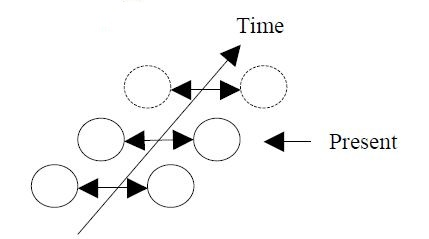
\includegraphics[scale=0.5]{interpersonal.jpg}
\caption{Eksisterende relasjon og avbrudd}
\label{interpersonal}
\end{figure}

\noindent
Avbrudd kan også ha effekter på andre mennesker som befinner seg på samme lokasjon som den som blir avbrutt. Dette illustreres i figur \ref{collateral}, hvor interaksjonen mellom aktør D (avbryter) og aktør B (den som avbrytes) også påvirker aktører A og C.
\begin{figure}[H]
\centering
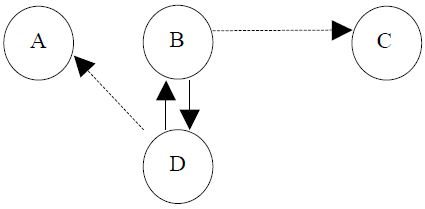
\includegraphics[scale=0.5]{collateral.jpg}
\caption{Lokasjonsbasert forstyrrelse}
\label{collateral}
\end{figure}

\noindent
En annen situasjon som kan oppstå er det Harr og Kaptelinin (2007) kaller frysing. Dersom aktører B og C utfører en oppgave ved synkron kommunikasjon, eksempelvis ansikt-til-ansikt eller per telefon, og aktør A avbryter aktør B, vil aktør C måtte vente til aktør B igjen blir tilgjengelig. 
\begin{figure}[H]
\centering
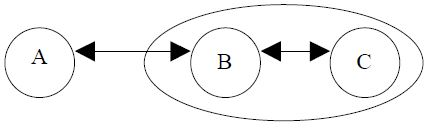
\includegraphics[scale=0.5]{frysing.jpg}
\caption{Frysing}
\label{frysing}
\end{figure}

\noindent
For en gruppe samarbeidende individer, vil oppgaver utført av et enkelt individ ofte være deler av den overordnete kollektive aktiviteten. Dermed vil forstyrrelsen av et individ sannsynligvis påvirke andre medlemmer i gruppen. Figur \ref{direkte} viser aktør B og aktør C som samarbeider om en gruppeoppgave GT, hvor GT er en del av den overordnete aktiviteten CA. Dersom aktør A avbryter aktør B, vil aktør C kanskje måtte dekke for aktør B, frem til B igjen blir tilgjengelig.
\begin{figure}[H]
\centering
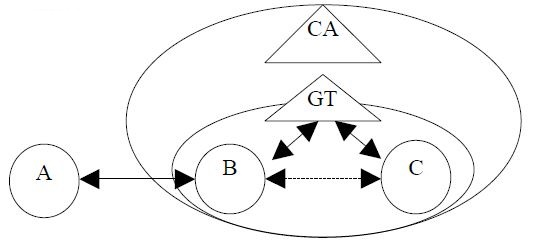
\includegraphics[scale=0.5]{coverme.jpg}
\caption{Samarbeid og avbrudd - direkte forstyrrelse}
\label{direkte}
\end{figure}

\noindent
Aktører B og C må ikke nødvendigvis kommunisere direkte, men aktør C kan være avhengig av tiden, innholdet og kvaliteten aktør Bs oppgave resulterer i. Dermed kan en forstyrrelse av aktør B også indirekte forstyrre aktør C.
\begin{figure}[H]
\centering
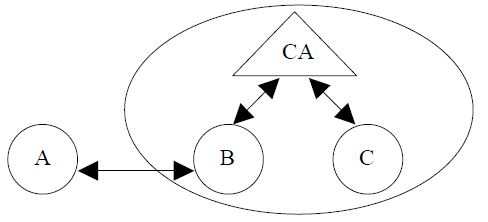
\includegraphics[scale=0.5]{dropball.jpg}
\caption{Samarbeid og avbrudd - indirekte forstyrrelse}
\label{indirekte}
\end{figure}

\noindent
Forskere som arbeider innen \emph{interruption value evaluation}-paradigmet tar utgangspunkt i at ikke alle avbrudd er dårlige, og at de ikke bør evalueres kun avhengig av hvordan de påvirker lokal kontekst, men også avhengig av hvor stor nytte de har. Målet er dermed å optimalisere individets beslutningstakingsprosess om hvordan han skal respondere på avbruddet. Den mest aktuelle teknikken for avbruddshåndtering vil derfor være forhåndsvisning av informasjon om avbruddet, hvem det er fra og hva det handler om, slik at individet selv kan reflektere over hvordan han/hun skal respondere basert på sin lokale kontekst. Dermed vil også det Grandhi og Jones (2010) kaller relasjonell kontekst være en del av avbruddskonteksten. Denne defineres som alle aspekter mellom den som avbryter og den som blir avbrutt, hvilken relasjon de har, hva avbruddet dreier seg om og deres tidligere interaksjonsmønstre.

\subsubsection{Utfordringer}
Harr og Kaptelinin (2007) påpeker tre fundamentale utfordringer ved avbruddshåndtering: (1) fare for å miste informasjon, (2) mindre privatliv og (3) utsettelse av oppgaver. For hver situasjon må individer finne den optimale balansen mellom isolasjon og tilgjengelighet, åpenhet og privatliv, og direkte eller utsatt håndtering av avbruddene.
\begingroup
\let\clearpage\relax
\section{Suksesskriterier ved implementering}
\label{chp: suksesskriterier}


\subsection{Brukbarhet}
\label{chp: brukbarhet}

Brukbarhet defineres i ISO 9241-11 \cite{Svanes08} som

\noindent
\begin{otherlanguage}{english}
\emph{the extent to which a product can be used by specified users to achieve specified goals with effectiveness, efficiency and satisfaction in a specified context of use.}
\end{otherlanguage}

\noindent
Brukbarhet er dermed et begrep som ikke kan måles generelt, men er relativt til bestemte brukere med bestemte mål i en spesifikk kontekst. Likevel kan man generelt definere noe som brukbart dersom det er funksjonelt, effektivt og tilfredsstillende \cite{Kuniavsky}. Et system er funksjonelt når det anses som nyttig av brukeren, og må dermed svare til de forventningene brukeren har til hva det skal gjøre, og faktisk gjøre det. Effektivitet kan måles som hvor raskt en er i stand til å utføre en oppgave med så lite feil som mulig. Det er vanskelig å konkretisere hva som gjør et system tilfredsstillende for en bruker, dette er individuelt og er en følelsesmessig respons ved bruk systemet \cite{Kuniavsky}. Ofte vil god design være avgjørende for om en bruker opplever systemet på en god måte, forutsett at det også er funksjonelt og effektivt. Designere av grensesnitt har gjennom årene kommet frem til en rekke reningslinjer for god design. Desverre er disse ofte blitt kritisert for å være både for spesifikke og ufullstendige \cite{mmi}. 
Interaktive applikasjoner og systemer vil spesielt hemmes av dårlig design dersom de allerede er vanskelige å lære og kompliserte å bruke. Slike systemer kan også føre til katastrofale utfall dersom kritisk informasjon ikke blir presentert på en effektiv måte. Det er derfor avgjørende å ha forståelse for hva slags informasjon brukeren trenger og hvordan denne skal presenteres \cite{Ebright10}. 

\subsubsection{Gestaltprinsippene}
Gestaltprinsippene har sitt navn fra det tyske \emph{gestalten}, som betyr "å forme". Prinsippene blir ofte referert til som lover, og det finnes mange varianter utviklet av forskjellige psykologer. Det de har til felles at de forklarer hvordan vi organiserer og tolker visuelle intrykk i områder og strukturer. Disse prinsippene beskriver blant annet virkningen av plassering av fokuspunkt, organisering av elementer, fargevalg, harmoni og enkelhet, og understeker at vi alle tolker visuelle inntrykk ut ifra egne erfaringer. 
Disse prinsippene ble i utgangspunktet brukt til å foreslå hvordan statiske visuelle elementer burde presenteres. I dag er det vanlig å ta hensyn til disse retningslinjene i design av blant annet skjermbilder \cite{Chang02}. 

\subsubsection{Affordance, konseptuelle modeller og begrensninger}
Vår forståelse av hvordan vi skal bruke en gjenstand første gang vi ser den beror på tre dimensjoner: konseptuell modell, begrensninger og \emph{affordance}. Ordet affordance ble innført av psykologen J. J. Gibson. Det finnes ingen norsk oversettelse, men begrepet refererer til hva slags handling en gjenstand signaliserer når du ser den for første gang \cite{Norman99}.

\noindent
Det skilles mellom ekte affordance og oppfattet affordance, hvor det først og fremst er oppfattet affordance vi kan kontrollere i skjermdesign. Ekte affordance vil med tanke på datamaskiner være tastatur, skjerm, knapper og musepeker som signaliserer handlinger som berøring, peking, trykking og å se på. Ekte affordance finnes alstå uavhengig av hva som vises på skjermen. Det som vises på skjermen er visuelle tilbakemeldinger som viser hva vi kan gjøre, altså oppfattet affordance \cite{Norman99}.

\noindent
Affordance blir ofte forvekslet med begrensninger og konvensjoner. Vi kan si å ha tre typer begrensninger:
\begin{enumerate}
\item Fysiske begrensninger, som har sammenheng med ekte affordance. Et eksempel på dette kan være at det er ikke mulig å flytte musepekeren utenfor skjermen. 
\item Logiske begrensninger er sterkt knyttet til en god konseptuell modell. Et eksempel på dette er hvordan brukeren vet at den må skrolle for å se resten av siden.
\item Kulturelle begrensninger er tillært og deles av en gruppe mennesker, eksempelvis hva det betyr når markøren skifter form.
\end{enumerate}
En konvensjon er en kulturell begrensning som har utviklet seg over tid, og som forbyr noe og oppfordrer til noe annet. Slike konvensjoner er langsomme, i den betydning at det tar lang tid før de blir adoptert, og når de først er blitt det, tar det vel så lang tid før de forsvinner \cite{Norman99}.

\noindent
Spesielt logiske og kulturelle begrensninger er sterke virkemidler innen skjermdesign, da designere er mer opptatt av hva brukerene oppfatter som mulig, fremfor hva som faktisk er sant. Tilbakemeldinger og reaksjoner fra skjermen hjelper oss å forstå hva vi kan og skal gjøre \cite{Norman99}.
\endgroup
\subsection{Workarounds}
\label{chp: workarounds}

Workarounds defineres av Kobayashi (2005) som \emph{"informal temporary practices for handling exceptions to normal workflow"}. Direkte oversatt til norsk betyr det "å jobbe rundt", eller å finne midlertidige løsninger.
\noindent
Workarounds kan være nødvendig når det oppstår akutte situasjoner hvor man ikke har nødvendige ressurser tilgjengelig, eller de kan oppstå som følge av sperrer i et system. Disse sperrene kan være tilsiktede, eller utilsiktede. Et eksempel på førstnevnte finner vi i \cite{Vogelsmeier08}, hvor sykepleiere ikke kan bestille doser av medisiner høyere enn det som er anbefalt. I tilfeller hvor høyere doser likevel var skrevet ut av lege, bestilte pleierene bare flere doser. 
Et annet eksempel på en workaround er gitt av Klemets, Evjemo og Kristiansen (2013), som beskriver hvordan sykepleiere fordeler ansvar for pasienter når de skal gå til lunsj. I utgangspunktet fordeles ansvar for pasienter gjennom en bemanningsplan som konfigureres i en applikasjon kjørende på en PC i sengeområdet. Å endre på denne planen krever merarbeid, og noen sykepleiere velger derfor å ikke gjøre endringene, men heller gi muntlig beskjed til kolleger om at en går til lunsj. Dette fører til at telefonene ringer under lunsjpausen.

\noindent
Vogelsmeier (2008) beskriver workarounds som førstegrads problemløsing i den forstand at man lager mekanismer for å jobbe rundt problemer, uten å forsøke å løse den underliggende årsaken til at problemet oppsto.
Dersom workarounds oppstår som konsekvens av utilsiktede sperrer, eller der systemet er for rigid i forhold til sykepleierenes arbeidsmønster slik at systemet ikke støtter opp om arbeidet på en tilfredstillende måte, er dette svært uheldig. Dette kan i verste fall føre til livstruende situasjoner.
Selv om slike workarounds er vanlige i medisinske settinger, er de som beskrevet ikke nødvendigvis effektive og vellykkede. Workarounds som gir organisatoriske løsninger for unntak som stadig gjentar seg, og dermed reduserer den kognitive innsatsen som kreves for å håndtere nye krisesituasjoner, vil ofte være suksessfulle. Workarounds som derimot gir ringvirkninger av ustabilitet i resten av organisasjonen, kan sies å være lite suksessfulle, selv om de løser problemet der og da \cite{Kobayashi05}.
\subsection{Utfordringer med CSCW}
\label{chp: utfordringerMedCSCW}

Mange CSCW-systemer faller til kort når det kommer til forventningene til deres suksess. Dette kommer gjerne til syne ved at de tiltenkte brukerene ganske enkelt unngår å bruke systemet, eller at de stadig må lage midlertidige løsninger (workarounds) for å få gejnnomført arbeidsoppgavene sine. Spesielt to grunner til dette er knyttet til kompleksiteten rundt å utvikle multibrukersystemer, som brukes samtidig av mange brukere på forskjellige nivåer og med forskjellige behov og perspektiver.

\noindent
For det første er det ofte manglede kunnskap om CSCW (multibruker-)systemer, i motsetning til enkeltbruker-systemer. En typisk CSCW-applikasjon eller system vil vanligvis bli brukt av et vidt spekter av forskjellige brukere, med forskjellig bakgrunn, erfaringer og forhold til bruk av informasjonssystemer generelt. Beslutningstakere, ofte ledere, vil ha en intuisjon for hva som vil være fordelaktige for brukere som en selv. Desverre kan de fort overse funksjoner som andre brukere vil ha nytte av, spesielt for fuksjoner som vil før til merarbeid for dem selv. 

\noindent
Det andre er at det vanskelig å lære fra tidligere feil, da CSCW-systemer er svært komplekse og unike for hvert enkelt tilfelle, noe som vanskeliggjør evaluering i ettertid. Det er også vanskelig, om ikke umulig å gjenskape miljøene og forholdene som er essensielle i den virekelige konteksten hvor et CSCW-system skal implementeres i et laboratorium. for ikke å snakke om utfordringene ved å gjøre feltobservasjoner, grunnet blandt annet variasjon i gruppesammensettning og miljømessige faktorer.


\subsection{Motstand mot endring}
\label{chp: motstand}

Implementering av nye informasjonssystemer kan by på utfordringer for ledelsen og utviklere dersom de ansatte viser motstand mot endringen. 
En slik endring vil påvirke menneskene som jobber der, deres sosiale relasjoner og forholdet mellom mennesker i og utenfor organisasjonen. Derfor kan det oppstå motstand uavhengig av hvor godt systemet som implementeres er, og i hvor stor grad de ansatte har fått bidra i utviklingen i form av medvirkning \cite{Jacobsen12}. Cavaye (1995) kaller denne motstanden for mellomliggende variabler, og understreker at sli
orhold til designer/utvikler og deres innspill blir hørt. Det finnes flere årsaker til slik motstand mot endring, og vi vil her forklare noen av dem. 

\subsubsection{Faglig uenighet}
De ansatte kan være faglig uenige i selve endringen. Verken analyser av dagens situasjon, behovet for endring eller selve endringen er klare og objektive størrelser, og det er derfor også rom for uenigheter rundt det faktiske behovet for endring, og hvorvidt endringen som gjennomføres er den rette løsningen på problemet. \cite{Jacobsen12}

\subsubsection{Merarbeid}
En endring i seg selv kan kreve ekstraarbeid fra de ansatte, spesielt i en overgangsfase. Det kan være mye nytt å sette seg inn i og lære, noe som krever en ekstra innsats, ofte uten tilstrekkelig kompensasjon, noe mange stiller seg negative til. Slikt ekstraarbeid kan i tillegg til å lære noe nytt innebære at man må avlære de gamle måtene å jobbe på. \cite{Jacobsen12}

\subsubsection{Systemet som en trussel}
Dersom brukerene ser på det nye systemet som en trussel mot deres nåværende kontroll over eget arbeid, eller deres posisjon i form av deres ekspertise, vil de mest sannsynlig motsette seg endringen det nye systement representerer. \cite{Cavaye95}

\subsubsection{Grad av medvirkning}
Motstand kan også oppstå dersom det faktiske nivået av medvirkning avviker fra det nivået brukeren ønsker seg. Dette gjelder ikke bare dersom nivået er lavere, men også dersom nivået av medvirkning blir høyere enn det brukeren så for seg i utgangspunktet. Det er derfor ikke tilstrekkelig med medvirkning i seg selv, den må også møte brukerenes forventninger. \cite{Cavaye95}

\noindent
Jacobsen(2012) hevder at indre motivasjon og involvering de ansatte, slik at de føler seg som medeiere i endringsprosessen er avgjørende for å få de ansatte motivert for endringen og dermed redusere overnevnte motstand. Bred deltagelse på denne måten gir den enkelte ansatte opplevelsen av at den er med på å forme sin egen fremtid, og at dette vil skape en aksept og forståelse for usikkerheten som er assosiert med en hver endring.
\subsection{Brukermedvirkning og deltagende design}
\label{chp: medvirkning}

\subsubsection{Brukermedvirkning}
Uttrykket \emph{brukermedvirkning} er sammensatt av to aspekter, \emph{bruker} og \emph{medvirkning}. For å forstå hva brukermedvirkning egentlig er må vi forstå de to aspektene enkeltvis. Vi må anerkjenne at det finnes flere typer \emph{brukere}. Det kan være toppledelsen, som bruker systemets output i sine analyser og strategiske avgjørelser. Det kan være mellomledere som er ansvarlig for, og overvåker, avdelinger som bruker systemet. Til sist har vi de ansatte som bruker systemet i sitt daglige arbeid. Det er ofte naturlig at alle brukergruppene tar del i utviklingsprosessen i større eller mindre grad. Toppledelsen må kanskje godkjenne systemet, og kan ha meninger om hva slags rapporter det skal generere. Mellomledelsen og andre ansatte kan bidra med innsikt i dagens arbeidsrutiner, problemer og workarounds, samt kravspesifikasjoner, ønsker til design og testing. Vi må også forstå at \emph{medvirkning} ikke er det samme som involvering, selv om de to uttrykkene ofte blir brukt om hverandre. I Cavaye (1995) finner vi definisjonene av (bruker)medvirkning og involvering som henholdsvis \emph{"a set of operations and activities performed by users"} i løpet av utviklingsprosessen, og \emph{"subjective psycological state"} som påvirker brukernes forestillinger, og dermed systemets grad av suksess.

\noindent
Brukermedvirkning finner vi i mange former og på flere nivåer. Som vi ser i tabell \ref{Beskrivelse av brukermedvirkning} kan medvirkning beskrives ved hjelp av flere attributter. 

\begin{table}[H]
\caption{Beskrivelse av brukermedvikrning (hentet fra Cavaye (1995))}
%\centering
\begin{tabular}{c c}
\hline\hline
\textbf{Medvirkningsattributter} & \textbf{Mulige verdier} \\ [2ex]
\hline
& alle brukere \\[-1ex]
\raisebox{1.5ex}{Type} & representativt utvalg av brukere \\ [2ex]
\hline
& rådgivende \\ & signeringsansvar  \\
\raisebox{2ex}{Grad} & del av teamet \\ & fullt ansvar \\ [2ex]
\hline
& teknisk design \\
\raisebox{1.5ex}{Innhold} & sosialt og teknisk design \\ [2ex]
\hline
& prosjektdefinering  \\ & kravspesifikasjon  \\
\raisebox{2ex}{Område} & utvikling \\ & testing \\ [2ex]
\hline
& formell \\
\raisebox{1.5ex}{Formalitet} & uformell \\ [2ex]
\hline
& innspill ignorert \\
\raisebox{2ex}{Innflytelse} & bidrag tatt i betraktning  \\ & innspill tas seriøst \\
\hline
\end{tabular}
\label{Beskrivelse av brukermedvirkning}
\end{table}

\begin{itemize}
\item Type medvirkning beskriver andelen av brukere som faktisk blir inkudert. Det er ikke alltid det lar seg gjøre å inkludere alle brukere i praksis. Da er det viktig å etterstrebe å ha et representativt utvalg av disse med i prosessen.
\item Grad av medvirkning viser til at brukere har forskjellig grad av ansvar gjennon sin medvirkning.
\item Innholdet i medvirkningen refererer til det faktum at brukerne kan involveres i forskjellige aspekter av utviklingsprosessen. Det er vanlig at brukere involveres i aktiviteter som forbereder det tekniske designet av systemet, men de kan også involveres i det sosiale designet, det vil si de menneskelige og sosiale effektene systemet vil ha.
\item Området medvirkningen angår vil variere gjennom de forskjellige fasene av utviklingsprosessen. Medvirkning fra brukerne er mer vanlig i forbindelse med å sette rammer for prosjektet, kravsspesifikasjon og testing enn gjennom selve utviklingen og kodingen av systemet.
\item Medvirkningen kan være formell, ved bruk av formelle grupper og team, eller uformell, med tilfeldige diskusjoner og oppgaver.
\item Innflytelsen brukerene faktisk har kan variere, og innspill fra disse kan vektlegges i forskjellig grad av utviklerene, alt fra å bli totalt ignorert til å bli tatt svært seriøst. Dette betyr at det kan legges ned mye ressurser i å la brukerne få komme med innspill, men at virkningen av disse beror på i hvilken grad disse blir tatt hensyn til.
\end{itemize}

\noindent
I mange år ble det sett som en selvfølge at brukermedvirkning hadde en signinfikant positiv effekt på en eventuell suksess for et informsjonsystem. Empiriske studier kan imidlertid ikke bevise at det alltid er en slik sammenheng \cite{Cavaye95}. Dermed ser det ut til at brukermedvirkning hverken er tilstrekkelig eller ytterst nødvendig for å garantere suksess for et informasjonsystem. 
Det er flere grunner til dette, sett fra både designers/utviklers og brukerens side. For det første har forholdet mellom bruker og designer/utvikler stor innvirkning på effekten av medvirkningen. Forskjeller i bakgrunn, erfaring og perspektiver kan føre til konflikter som igjen preger effekten av medvirkningen på en negativ måte. For det andre spiller det ingen rolle i hvor stor grad brukerne medvirker i prosessen dersom deres innspill blir ignorert. For det tredje vil de ansattes motstand mot endring kunne resultere i ubrukte systemer, eller bevisst sabotasje av implementeringen og endringsprosessen. Som beskrevet i avsnitt \ref{chp: motstand}, vil motstand mot endring kunne reduseres ved god informasjon og involvering (til forskjell fra medvirkning) av de ansatte. Dette må ikke sees som en motsetning til Cavaye (1995)s påstand om at medvirkning ikke er en garanti for suksess. Dette fordi informasjon til og involvering av de ansatte ikke nødvendigvis behøver å inkludere medvirkning, og fordi selv med medvirkning og innspill fra de ansatte er en ikke garantert å redusere motstanden tilstrekkelig til å sikre en suksessfull implementering av det nye systemet \cite{Cavaye95}.

\subsubsection{Deltagende design}
\label{dd}
Deltagende design er én av mange teknikker for å oppnå brukermedvikning.
Interessen for denne teknikken blir stadig større, og sees på som en god måte å blant annet sikre gode innspill fra brukere (for blant annet analyse av dagens situasjon), gjensidig læring og bedring av arbeidsrutiner.

\noindent
Vi kan dele utvikling av informasjonsystemer i tre aspekter: analyse, design og praksis. Det kan være vanskelig å kombinere alle tre samtidig, og tidligere ble det sett på som svært positivt om man greide å kombinere to av disse. Mogensen og Trigg (1992) ser i sin studie på muligheten for å kombinere alle tre aspektene samtidig (figur \ref{Challenge_PD}).

\begin{figure}[H]
\centering
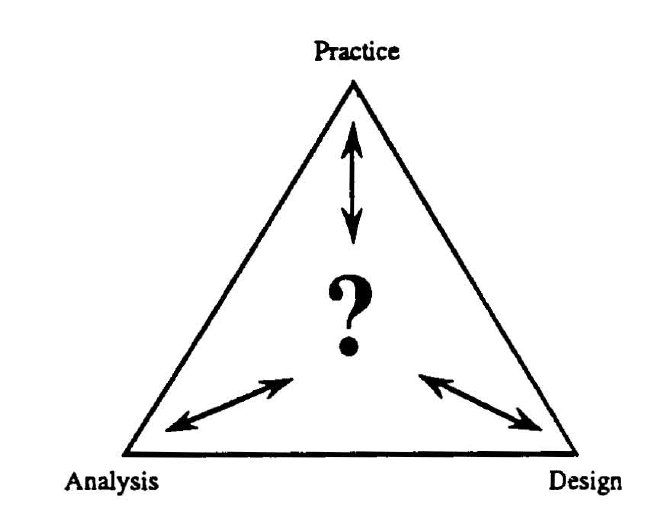
\includegraphics[scale=0.3]{Challenge_PD.jpg}
\caption{Hvordan kombinere alle?}
\label{Challenge_PD}
\end{figure}

\noindent
Ifølge \cite{Mogensen92} er det flere måter å oppnå større medvirkning på. Én teknikk er \emph{fremtidsworkshops}, der en ønsker diskusjon rundt mulige fremtidige løsninger på nåværende problemer, identifisert av brukerne selv. En annen teknikk er workshops hvor en bruker mock-ups og prototyper for å trigge diskusjon om mulige fremtidige teknologier og løsninger. Uavhengig av valgt teknikk vil graden av relevans til dagens praksis være avgjørende for workshopens suksess. Felles for de to er at de tar i bruk kontekstuelle artefakter (artefakter medbrakt av fasilitator som brukerene selv setter i kontekst).

\noindent
Mogensen og Trigg (1992) konkluderer med at bruk av kontekstuelle artefakter og hvor alle de tre faktorene, analyse, praksis og design er tilstede kan lede til nettopp et slikt ønsket samspill som vist i figur \ref{Artifacts_PD}. De argumenterer for at bruk av artefakter under en workshop ikke bare gir innspill på design - deltagende design, men at de også kan trigge diskusjoner som gir utviklerene bedre innsyn i dagens praksis, problemer og workarounds - deltagende analyse. 

\noindent
Deltagende design på denne måten, med bruk av kontekstuelle artefakter, gir derfor forskere/utviklere en dypere forståelse av hva som er problemområdene, og hvordan brukerne selv oppfatter dagens situasjon. Det gir også brukerne mulighet til større bevissthet rundt egne arbeidsmetoder, -rutiner og workarounds.

\begin{figure}[H]
\centering
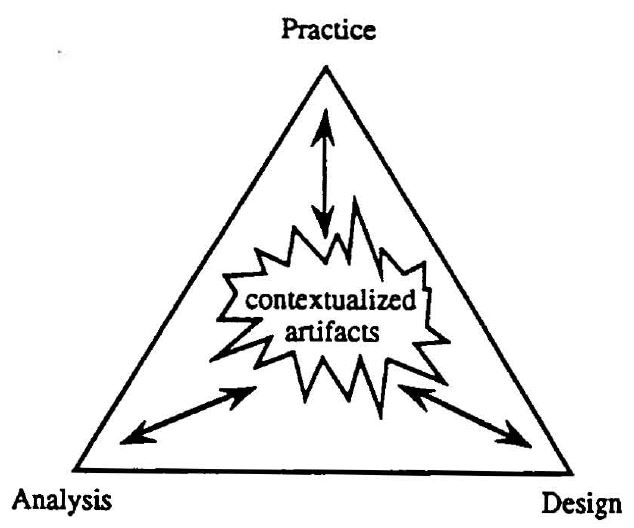
\includegraphics[scale=0.3]{Artifacts_PD.jpg}
\caption{Kontekstuelle artefakter støtter samspillet mellom de tre perspektivene}
\label{Artifacts_PD}
\end{figure}
\chapter{Forskningsmetode og hensikt}
\label{chp:forskningsmetode}

“I just want to develop a computer-based system” (Oates, 2006)

\noindent
Ifølge Oates (2006) er design og utvikling av ethvert databasert produkt en form for forskning som krever innsamling av data, analyse og konklusjon. For å utvikle et produkt eller system som skal utføre gitte oppgaver er det viktig å besvare hva disse oppgavene er, og hvorfor de er viktige. Dette besvares ved å samle informasjon om hva man ønsker av systemet, generere egen data som dokumenterer hvordan og hvorfor man designer og implementerer produktet, og deretter brukerteste og evaluere det. Vi vil i dette kapittelet først presentere hensikten med prosjektet før vi går i detalj på hvilke tilnærminger og metoder vi har valgt for å besvare forskningsspørsmålene.


\section{Hensikt}
\label{chp: hensikt}

Hensikten gjenspeiler den underliggende grunnen til å gjøre forskning, hva som gjør den interessant og hvorfor den er viktig eller nyttig. Videre kan man se på hvorfor man ønsker å forske på noe \cite{Oates}. 

\noindent
Motivasjonen for oppgaven var innledningsvis å avdekke fordeler og utfordringer i det eksisterende pasientsignalsystemet, og hvordan det kunne videreutvikles for å bedre støtte sykepleierenes behov. En gjennomgang av tidligere arbeid ga en bredere forståelse av forskningsområdet, og vi ønsket derfor å utdype problemstillingen. Vi formulerte to forskningsspørsmål som søkte svar på hvorvidt informasjon om kollegers aktiviteter og tilgjengelighet er nyttig, og hvordan slik informasjon kan kommuniseres på en hensiktsmessig måte. Da tidligere arbeid viste at avbrytelser kan ha en negativ effekt på sykepleieres arbeid, ønsket vi samtidig å undersøke hvordan systemet kan endres for å redusere eventuelle negative effekter.

\subsubsection{Forskningsspørsmål}
Vi har formulert to spørsmål som vi søker svar på gjennom denne oppgaven. Disse er som følger:

\begin{enumerate}
\item Er informasjon om kollegers aktiviteter og tilgjengelighet nyttig for sykepleiere, og hvordan kan slik informasjon distribueres på en hensiktsmessig måte? 
\item Hvordan kan systemet endres for å begrense potensielle negative effekter ved avbrytelser?
\end{enumerate}

\section{Prosess}
\label{chp: prosess}

Prosessen i et forskningsprosjekt kan beskrives som sekvensen av aktiviteter som utføres i løpet av prosjektets varighet \cite{Oates}. Vi vil nå gjøre rede for de metodene og tilnærmingene vi har valgt i vår prosess.

\subsection{Paradigme}
Et paradigme er et sett felles antakelser om, eller måter å tenke på, noen aspekter av verden \cite{Oates}. Innen samfunnsforskningen fremstår kvalitativ og kvantitativ forskning som to vesentlige tenkemåter, eller paradigmer, når det gjelder hvordan man kan framskaffe eller generere informasjon om samfunnet, for deretter å analysere det (Tjora, 2010).
[SKRIV OM KVALITATIV vs KVANTITATIV, INDUKTIV, DEDUKTIV OG ABDUKTIV]

\subsection{Litteraturstudie}
Teorien vi har lagt frem i kapittel \ref{chp:teori} er basert på et litteraturstudie gjort innledningsvis i arbeidet. For å definere forskningsspørsmålene knyttet til oppgaven, analyserte vi i første omgang tidligere arbeid gjort av Klemets, Evjemo og Kristiansen (2013). Dette ga oss et inntrykk av forskningsområdet og utfordringene knyttet til det eksisterende pasientsignalsystemet. 

\subsection{Dokumentstudie}

\subsection{Prototype}
Ifølge Schneiderman og Plaisant (2010) mislykkes mange utviklingsprosjekter i å nå sine mål, i stor grad grunnet dårlig kommunikasjon mellom utviklere og brukere. Suksessfulle utviklere legger derfor stor vekt på å forstå kundens behov og krav. 
Brukersentrert design gir systemer som genererer færre problemer under utviklingen, og lavere vedlikeholdskostnader. De er enklere å lære, gir raskere ytelse og vesentlig mindre feil \cite{mmi}.
Prototyping er en velkjent måte å utforske og uttrykke design for interaktive systemer. 

\tikzstyle{mybox} = [draw=black, fill=white, very thick,
    rectangle, inner sep=10pt, inner ysep=20pt, rounded corners]
\tikzstyle{fancytitle} =[fill=black, text=white]
\begin{tikzpicture}
\node [mybox] (box){%
    \begin{minipage}{0.9\textwidth}
      En prototype defineres som enhver representasjon av en designidé, uavhengig av medium \cite{Houde97}.
    \end{minipage}
};
\node[fancytitle, rounded corners, right=10pt] at (box.north west) {Definisjon av prototype};
\end{tikzpicture}%





%% include here the other chapters

%\renewcommand*{\bibname}{References}
%\bibliographystyle{alpha}
%\bibliography{main}

\begin{thebibliography}{99}

\bibitem{Klemets13}
Klemets, J. and Kristiansen, L., 2013
\emph{Extended Communication Possibilities for Nurses: Taking Context into Consideration}
IOS Press
  
% DENNE ER IKKE PUBLISERT OG KAN DERFOR IKKE BRUKES SOM KILDE
%\bibitem{Evjemo}
%Evjemo, T. E. and Klemets, J., 
%\emph{Maintaining Awareness: Nurses’ Handling of Interruptions in the Wireless Nurse Call System} Norwegian University of Science and Technology

\bibitem{Bardram04}
Bardram, J. E. and Hansen T. R., 2004
\emph{The AWARE Architecture: Supporting Context-Mediated Social Awareness in Mobile Cooperation}

\bibitem{KlemetsRedundancy}
Klemets, J., Evjemo, T. E. and Kristiansen, L.
\emph{Designing for redundancy: Nurses Experiences with the Wireless Nurse Call System}

\bibitem{Dourish92}
Dourish, P. and Bellotti, V., 1992
\emph{Awareness and Coordination in Shared Workspaces}
CSCW 92 Proceedings

\bibitem{Heath02}
Heath, D. et al., 2002
\emph{Configuring Awareness}
CSCW 11: 317-347, 2002

\bibitem{Gutwin04}
Gutwin, C., Penner, R., and Schneider, K., 2004
\emph{Group Awareness in Distributed Software Development}
CSCW`04, November 6-10, 2004 Chicago, Illinois, USA

\bibitem{Scholl07}
Scholl, J., Hasvold, P., Henriksen, E. and Ellingsen, G., 2007
\emph {Managing communication availability and interruptions: a study of mobile communication in an oncology department.} 
In Proceedings of the 5th international conference on Pervasive computing(PERVASIVE'07), Anthony LaMarca, Marc Langheinrich, and Khai N. Truong (Eds.). Springer-Verlag, Berlin, Heidelberg, 234-250.

\bibitem{McGillis10}
McGillis Hall L, Pedersen C, Fairley L., 2010
\emph {Losing the moment: understanding interruptions to nurses' work.}
J Nurs Adm. 2010;40:169-176.

\bibitem{Parker00}
Parker J, Coiera E., 2000
\emph {Improving clinical communication: a view from psychology.} 
J Am Med Inform Assoc 2000;7, 453–61.

\bibitem{Grundgeiger09}
Grundgeiger, T., Sanderson, P., 2009
\emph {Interruptions in healthcare: Theoretical views}
International Journal of Medical Informatics, Volume 78, Issue 5, May 2009, 293–307.

\bibitem{Ebright10}
Ebright, P., 2010
\emph {The Complex Work of RNs: Implications for Healthy Work Environments}
OJIN: The Online Journal of Issues in Nursing Vol. 15, No. 1, Manuscript 4.

\bibitem{Grandhi10}
Grandhi, S., Jones, Q., 2010
\emph {Technology-mediated interruption management} Int. J. Hum.-Comput. Stud. 68, 5, May 2010, 288-306.

\bibitem{Endsly95}
Endsly, M. R., 1995
\emph{Toward a Theory of Situation Awareness in Dynamic Systems}
Human Factors: The Journal of the Human Factors and Ergonomic Society, Mar 1, 1995 37:32

\bibitem{Schmidt02}
Schmidt, K., 2002
\emph{The Problem With 'Awareness'}
Computer Supported Cooperative Work 11: 285-298, 2002
2002 Kluwer Academic Publishers

\bibitem{Gross13}
Gross, T., 2013
\emph{Supporting Efforstless Coordination: 25 Years of Awareness Research}
Computer Supported Cooperative Work
Published online: 23 June 2013

\bibitem{Klemets12}
Klemets, J., Kristiansen, L., 2012
\emph{A Pervasive System for Communicationg Urgency Cues to Health Care Workers}
24th International Conference of the European Federation for Medical Informatics

\bibitem{mmi}
Shneiderman, B., Plaisant, C., 2010
\emph{Designing the User Interface: strategies for effective human-computer interaction}
Pearson - fifth edition, Pearson Education, Inc.

\bibitem{Chang02}
Chang, D., Dooley, L. and Tuovien, J. E., 2001
\emph{Gestalt Theory in Visual Screen Design - A New Look at an Old Subject}
Presented at the Seventh World Conference on Computers in Education, Copenhagen, July 29 - August 3, 2001

\bibitem{Norman99}
Norman, D. A., 1999
\emph{Affordance, Conventions and Design}
Interactions 6, no.3, 38-43, 1999

\bibitem{Randell}
Randell, R., Wilson, S., Woodward, P., Galliers, J., 2010
\emph{Beyond handover: supporting awareness for continuous coverage} 
Cognition, Technology and Work, 12: 271-283, 2010 

\bibitem{Tjora}
Tjora, A., 2010 
\emph{Kvaltitative forskningsmetoder i praksis} 
Oslo: Gyldendal Akademisk

\bibitem{Oates}
Oates, B.J., 2006 
\emph{Researching Information Systems and Computing} 
SAGE Publicatioons Ltd.

\bibitem{Seland}
Svanæs, D., Seland, G., 2004 
\emph{Putting the Users Center Stage: Role Playing and Low-fi Prototyping Enable End Users to Design Mobile Systems} 
CHI 2004, 6:479-486

\bibitem{Svanes08}
Svanæs, D., Alsos, O., Dahl, Y., 2010
\emph{Usability testing of mobile ICT for clinical settings: Methodological and practical challenges}
International Journal of Medical Informatics, Volume 79, Issue 4, April 2010, pp. 24-34.

\bibitem{Nemeth04}
Nemeth, C., Cook, R., O'Connor, M., Klock, P., 2004
\emph{Using Cognitive Artifacts to Understand Distributed Cognition}
Systems, Man and Cybernetics, Part A: Systems and Humans, IEEE Transactions on , vol.34, no.6, pp.726-735, Nov. 2004

\bibitem{Grundin88}
Grundin, J., 1988
\emph{Why CSCW applications fail: problems in the design and evaluationof organizational interfaces}
Proceedings of the 1988 ACM conference on Computer-supported cooperative work (pp. 85-93). ACM

\bibitem{Berg99}
Berg, M., 1999
\emph{Patient care information systems and health care work: a sociotechnical approach}
International journal of medical informatics, 55(2), 87-101.

\bibitem{Harr07}
Harr, R., Kaptelinin, V., 2007
\emph{Unpacking the Social Dimension of External Interruptions}
Proceedings of the 2007 international ACM conference on Supporting group work (GROUP '07). ACM, New York, NY, USA, 399-408.

\bibitem{McCrickard03}
McCrickard, D. S., Chewar, C. M., Somervell, J. P., Ndiwalana, A., 2003
\emph{A model for notification systems evaluation—assessing user goals for multitasking activity}
ACM Trans. Comput.-Hum. Interact. 10, 4 (December 2003), 312-338.

\bibitem{Erickson00}
Erickson, T., Kellogg, W. A., 2000. 
\emph{Social translucence: an approach to designing systems that support social processes} ACM Trans. Comput.-Hum. Interact. 7, 1 (March 2000), 59-83.

\bibitem{Mogensen92}
Mogensen, M., Trigg, R. H., 1992.
\emph{Using artifacts as triggers for participatory analysis}
In PDC'92: Proceedings of the Participatory Design Conference. M.j.Muller, S.Khun and J.A.Meskill (Eds.). Cambridge MA US, 6-7 November 1992

\bibitem{Cavaye95}
Cavaye, A. L. M., 1995
\emph{User participation in system development revisited}
Information \& Management 28 (1995) 311-323

\bibitem{Jacobsen12}
Jacobsen, D. I., 2012
\emph{Organisasjonsendringer og endringsledelse}
Fagbokforlaget Vigmostad \& Bjørke AS, 2.utgave 2012


\bibitem{Kobayashi05}
Kobayashi, M., Fussell, S. R., Xiao, Y., Seagull, F. J., 2005
\emph{Work Coordiantion, Workflow, and Workarounds in a Medical Context}
CHI 2005, April 2-7, 2005, Postland, Oregon, USA

\bibitem{Kuniavsky}
Kuniavsky, M., 2003 
\emph{Observing the User Experience: A Practitioner's Guide to User Research}
Morgan Kaufmann Publishers Inc., San Francisco, CA, USA.


\end{thebibliography}

%% Uncomment the following if you have any appendix
% \appendix
% \addtocontents{toc}{%
%  \protect\vspace{1em}% 
%  \protect\noindent \bfseries \appendixtocname\protect\par
%  \protect\vspace{-.5em}%
% }
% \renewcommand{\chaptername}{\appendixname}
%% include below possible appendices (chapters)


\end{document} 
